\documentclass[compress,usenames,dvipsnames]{beamer}
\usepackage{tikz}
\usepackage{adjustbox}
\usepackage{beramono}

\usepackage[utf8]{inputenc}
\usepackage{listings}
\usepackage{pgfplots}
\usepackage{courier}
\usepackage[ruled]{algorithm2e}
\usetheme{Warsaw}
\usecolortheme{crane}
\DeclareUnicodeCharacter{2212}{−}
\usepgfplotslibrary{groupplots,dateplot}
\usetikzlibrary{patterns,shapes.arrows,arrows,positioning,backgrounds,fit,chains,matrix}

\usefonttheme[onlymath]{serif}
\lstset{
    language=Python,
    basicstyle=\ttfamily,
    otherkeywords={self},             
    keywordstyle=\ttfamily\color{blue!90!black},
    keywords=[2]{True,False},
    keywords=[3]{ttk},
    keywords=[4]{yield},
    keywords=[5]{next},
    keywordstyle={[2]\ttfamily\color{orange}},
    keywordstyle={[3]\ttfamily\color{red!80!orange}},
    keywordstyle={[4]\ttfamily\color{blue!90!black}},
    keywordstyle={[5]\ttfamily\color{RubineRed}},
    emph={MyClass,__init__},          
    emphstyle=\ttfamily\color{red!80!black},    
    stringstyle=\color{green!80!black},
    showstringspaces=false            
}
\SetKwProg{Fn}{def}{\string:}{}
\SetKw{True}{True}
\SetKw{Break}{break}

\author{Wing}
\title{Asyncio Internals}  

\begin{document}
\date{\today} 

\frame[plain]{\titlepage} % [plain] means it doesn't show the section above the Header 

\frame[plain]{\frametitle{Table of contents}
    \small
    \tableofcontents[hideallsubsections]
}
\section{Generator}
\begin{frame}[plain]
    \frametitle{Generator internals}
    Secret: In cpython, generator = coroutine!
    \begin{itemize}
        \item {\lstinline{gen.send(?)}}
        \item {\lstinline{next(gen)}} $\equiv$ {\lstinline{gen.send(None)}}
        \item {\lstinline{gen.throw(exc)}}
        \item {\lstinline{yield}} $\Rightarrow$ ``pausing'' of coroutine
        \item closure
        \item stack frame in heap

    \end{itemize}
    demo {\lstinline{gen_send.py}}
\end{frame}

\section{Event loop}

\begin{frame}[plain, t, fragile]
    \frametitle{Event loop}
    \begin{center}
    \begin{adjustbox}{}
         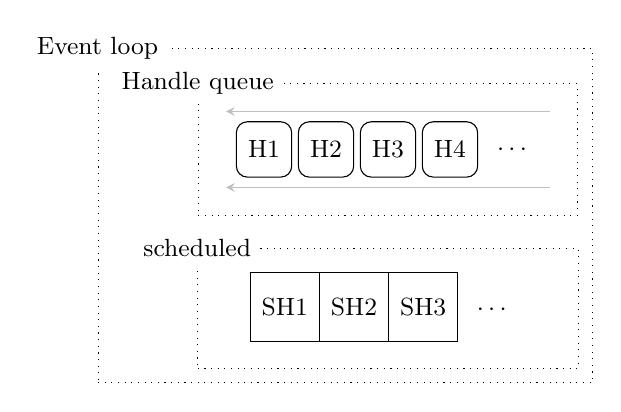
\begin{tikzpicture}[
    srrect/.style={rounded corners,minimum width=20pt,minimum height=20pt},
    sarr/.style={-stealth},font=\sffamily,font=\small,
    node distance=10pt
    ]
    \begin{scope}[start chain=going right,node distance=2pt,nodes={srrect,on chain}]
        \node[draw] (A2){H1};
        \node[draw] (B2){H2};
        \node[draw] (C2){H3};
        \node[draw] (D2){H4};
        \node[] (E2){$\cdots$};
    \end{scope}
    \node[fit=(A2) (E2)](F2){};
    \foreach \X in {north,south}
    {\draw[sarr,gray!50]  (F2.\X\space east) -- (F2.\X\space west);}
    \node[draw, fit=(F2), inner sep=10pt, dotted] (tq) {};
    \node[fill=white] (tqlabel) at (tq.north west) {Handle queue};
    \node[below=of tq, yshift=-20pt] (phan) {};
    \matrix[column sep=-\pgflinewidth, matrix of nodes, nodes={draw}, minimum size=25pt] (sh) at (phan.center) { SH1 & SH2 & SH3 & |[draw=none]|$\cdots$\\};
    \node[draw, dotted, fit= (sh) (tq.west |- phan.center) (tq.east |- phan.center), inner xsep=0pt, inner ysep=5pt] (shbox) {};
    \node[fill=white] (shlabel) at (shbox.north west) {scheduled};

    \node[draw, fit=(tq) (tqlabel) (shlabel) (shbox), inner sep=5pt, dotted] (eloop) {};
    \node[fill=white] (ellabel) at (eloop.north west) {Event loop};
\end{tikzpicture}

    \end{adjustbox}
    \end{center}
    {\ttfamily{Handle}} wraps \verb|Task.__step|
\end{frame}

\section{Task}

\begin{frame}[plain, t]
    \frametitle{Task}
    \begin{center}
    \begin{adjustbox}{margin=10pt}
             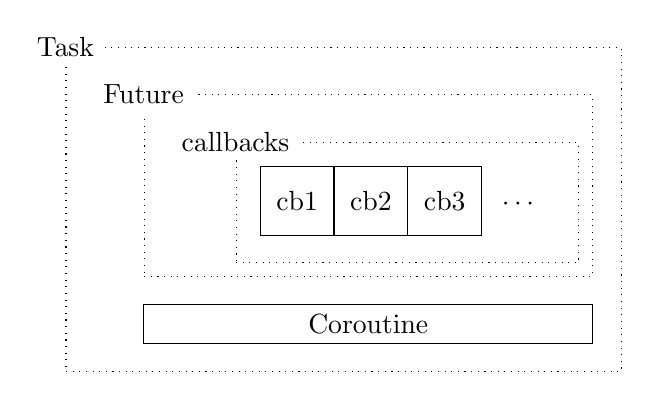
\begin{tikzpicture}[
array/.style={
    matrix of nodes,
    nodes={
        draw,
        text centered,
        text width=20pt,
        minimum size=25pt
    },
    column sep=-\pgflinewidth,
    nodes in empty cells,
    align=center,
    text centered
    },
    node distance=10pt
]

\matrix[array] (futcbarr) { cb1 & cb2 & cb3 &|[draw=none]|$\cdots$\\};
\node[draw, dotted, fit=(futcbarr), inner sep=5pt] (futcbbox) {};
\node[fill=white] (futcblabel) at (futcbbox.north west) {callbacks};
\node[draw, dotted, fit=(futcbarr) (futcblabel), inner sep=10pt] (futbox) {};
\node[fill=white] (futlabel) at (futbox.north west) {Future};
\node[below=of futbox] (coroboxcontent) {Coroutine};
\node[draw, inner sep=0, fit=(futbox.west |- coroboxcontent.center) (futbox.east |- coroboxcontent.center) (coroboxcontent)] (corobox) {};
\node[draw, dotted, fit=(corobox) (futbox) (futlabel), inner sep=10pt] (taskbox) {};
\node[fill=white] (tasklabel) at (taskbox.north west) {Task};

\end{tikzpicture}

    \end{adjustbox}
    \end{center}
\end{frame}

\section{Code flow}

\begin{frame}[plain, fragile]
    \frametitle{\lstinline{asyncio.run(main)}}
    \begin{lstlisting}
def run(main):
    loop = new_event_loop()
    return loop.run_until_complete(main)

class Loop:
    def run_until_complete(coro_or_fut):
        task = ensure_future(coro_or_fut)
        task.add_done_callback(<<stop loop>>)
        loop.run_forever()
        return task.result()

def ensure_future(coro_or_fut):
    if isinstance(coro_or_fut, Future)
        return coro_or_fut
    else:
        # coro
        return Task(coro_or_fut, loop=self)

    \end{lstlisting}
\end{frame}

\begin{frame}[plain, fragile]
    \frametitle{\lstinline{Task}}
    \begin{lstlisting}
class Task(Future):
    def __init__(self, coro, loop, ...):
        super().__init__(loop)
        ...
        self._coro = coro
        self._loop.call_soon(self.__step, ...)
    
    \end{lstlisting}
\end{frame}

\begin{frame}[plain, fragile]
    \frametitle{\lstinline{Future}}
    \scriptsize
    \begin{lstlisting}

class Future:
    def __init__(self, loop):
        self._loop = loop

    def __iter__(self):
        if not self.done():
            yield self  # future is blocking
        return self.result()

    def add_done_callback(self, fn, ...):
        if self.done():
            self._loop.call_soon(fn, self)
        else:
            self._callbacks.append((fn,))
    ...

    \end{lstlisting}
\end{frame}

\begin{frame}[plain, fragile]
    \frametitle{\lstinline{Future}}
    \scriptsize
    \begin{lstlisting}

class Future:
    ...

    def set_result(self, result):  # similar for set_exception
        self._result = result
        self._state = _FINISHED  # done
        self.__schedule_callbacks()

    def __schedule_callbacks(self):
        callbacks = self._callbacks[:]
        self._callbacks[:] = []  # clear callbacks
        for callback in callbacks:
            self._loop.call_soon(callback, self)

    def result(self):
        if self._exception is not None:
            raise self._exception
        return self._result
    \end{lstlisting}
\lstinline{__schedule_callbacks()} effectively moves all callbacks to \colorbox{SkyBlue}{Handle queue}
\end{frame}

\begin{frame}[plain]
    \frametitle{\lstinline{loop.call_soon(callback)}}
    \begin{algorithm}[H]
        \SetAlgoNoEnd
        \DontPrintSemicolon
        \Fn{\upshape \lstinline{call_soon(callback)}}{
            \lstinline{handle = Handle(callback)} \\
            \colorbox{SkyBlue}{Handle queue}\lstinline{.append(handle)} \\
            \Return \lstinline{handle}
        }
    \end{algorithm}
\end{frame}

\begin{frame}[plain, fragile]
    \frametitle{\lstinline{loop.run_forever()}}
    \begin{lstlisting}
def run_forever():
    while True:
        self._run_once()
        if self._stopping:
            break
    \end{lstlisting}
\end{frame}

\begin{frame}[plain]
    \frametitle{\lstinline{loop._run_once()}}
    \begin{algorithm}[H]
        \SetAlgoNoEnd
        \DontPrintSemicolon
        \Fn{\upshape \lstinline{_run_once()}}{
            \[\text{\lstinline{timeout}} = 
            \begin{cases}
                0, & \text{if \colorbox{SkyBlue}{Handle queue} is not empty} \\
                \text{minimal timeout}, & \text{if \colorbox{Lavender}{scheduled heap} is not empty} \\
                \text{None}, & \text{otherwise}
\end{cases}
\]

            // block if \lstinline{timeout is None} \\
            \lstinline{ev_list = self._selector.select(timeout)} \\
            \lstinline{self._process_events(ev_list)} \\
            \;
            \colorbox{SkyBlue}{Handle queue} \lstinline{+=} handles from \colorbox{Lavender}{scheduled heap} which the time is up \\
            \;
            \lstinline{handles =} pop all from \colorbox{SkyBlue}{Handle queue} \\
            \For{\upshape \lstinline{handle: handles}} {
                \lstinline{handle._run()} // runs \lstinline{task.__step}
            }
        }
    \end{algorithm}
\end{frame}

\begin{frame}[plain, fragile]
    \frametitle{\lstinline{Task.__step(exc)}}
    \scriptsize
    \begin{lstlisting}
def __step(exc):
    coro = self._coro
    try:
        result = coro.send(None)
    except StopIteration as exc:
        self.set_result(exc.value)
    except BaseException as exc:
        self.set_exception(exc)
    else:
        if result <<is a blocking future>>:
            result.add_done_callback(self.__wakeup)
    elif result is None:  # bare yield used
        self._loop.call_soon(self.__step)

def __wakeup(self, future):
    # check if cancelled or errored
    ...
    self.__step()
    \end{lstlisting}
\end{frame}

\begin{frame}[plain]
    \frametitle{\lstinline{demo}}
    \begin{itemize}
        \item \lstinline{run_once_demo.py}
        \item \lstinline{timeout_zero_future.py}
    \end{itemize}

\end{frame}

\section{References}
\begin{frame}[fragile,plain]\frametitle{References}
    \begin{thebibliography}{9}
        \bibitem{1} 
        Talk by Saúl Ibarra Corretgé in PyGrunn 2014
        \url{https://www.youtube.com/watch?v=HppNu0-ANYw} 
    \end{thebibliography}
\end{frame}
\end{document}
